\begin{figure}[h!]
    \centering
    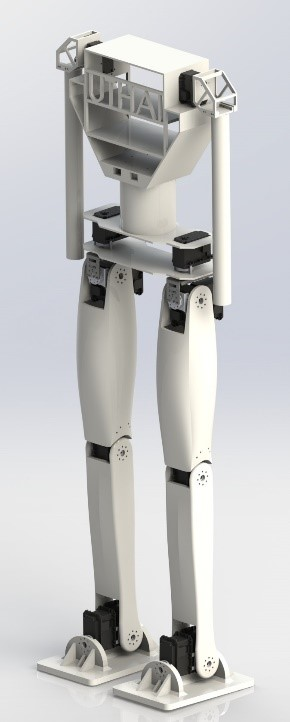
\includegraphics[width=0.2\textwidth]{chapter4/images/UTHAI_ver_1.jpg}
    \caption{โครงสร้างหุ่นยนต์ในโปรแกรม 3 มิติ}
    \label{fig:UTHAI_ver_1}
\end{figure}

โครงสร้างของหุ่นยนต์หลักๆจะแบ่งออกเป็น 2 ส่วนคือ ส่วนท่อนบนและส่วนท่อนล่างโดยส่วนท่อนบนจะประกอบไปด้วย 
เอว 1 ส่วน ลำตัว 1 ส่วน แขน 2 ส่วน และท่อนล่างจะประกอบไปด้วย สะโพก 1 ส่วน ขา 2 ส่วน น่อง 2 ส่วน ฝ่าเท้า 2 ส่วน 
ในการเลือกใช้วัสดุนั้นได้แสดงในตาราง 4.2

\begin{table}[ht]
	\centering
	\begin{tabular}{| l | l |}
		\hline
		ชิ้นส่วน & วัสดุที่ใช้ขึ้นรูป \\
        \hline
        ชิ้นส่วน & วัสดุที่ใช้ขึ้นรูป \\
        แขน	& ท่อคาร์บอนไฟเบอร์ ขนาด 30 มม. \\
        ลำตัว & เครื่องพิมพ์ 3 มิติ โดยใช้วัสดุ PLA \\
        เอว	& ท่อคาร์บอนไฟเบอร์ ขนาด 88 มม. \\
        สะโพก & อลูมิเนียมอัลลอยพับ \\
        น่อง & เครื่องพิมพ์ 3 มิติ โดยใช้วัสดุ PLA \\
        ขา & เครื่องพิมพ์ 3 มิติ โดยใช้วัสดุ PLA \\
        ฝ่าเท้า	& เครื่องพิมพ์ 3 มิติ โดยใช้วัสดุ PLA \\
	    \hline
	\end{tabular}
	\caption{ตารางแสดงวัสดุที่ใช้ขึ้นรูป UTHAI}
	\label{tab:UTHAI_material}
\end{table}

\clearpage
\subsection{การออกแบบโครงสร้างส่วนขา}
\subsubsection*{การออกแบบโครงสร้างส่วนขา(ครั้งที่1)}
การออกแบบโครงสร้างส่วนขาของหุ่นยนต์ฮิวมานอยด์ ได้ออกแบบโดยคำนึงถึงการขึ้นรูปด้วยเครื่องพิมพ์สามมิติ (3D Printer) 
แต่เนื่องจากว่าเครื่องพิมพ์สามมิติที่ใช้ในการผลิตนั้นมีขนาดที่เล็กกว่าขนาดที่จะพิมพ์จริงจึงต้องทำการแยกส่วนของขาออก
เป็นจำนวน 2 ส่วนในแต่ละในก้านต่อของขาท่อนบนและขาท่อนล่าง และหลังจากนั้นใช้การยึดชิ้นส่วนด้วยการตอกสลักเพื่อยึดติดชิ้นส่วนเข้าด้วยกัน
เพื่อให้มีความแข็งแรงมากกว่าการต่อแบบทั่วไป

\begin{figure}[h!]
    \centering
    \begin{subfigure}[b]{0.3\linewidth}
      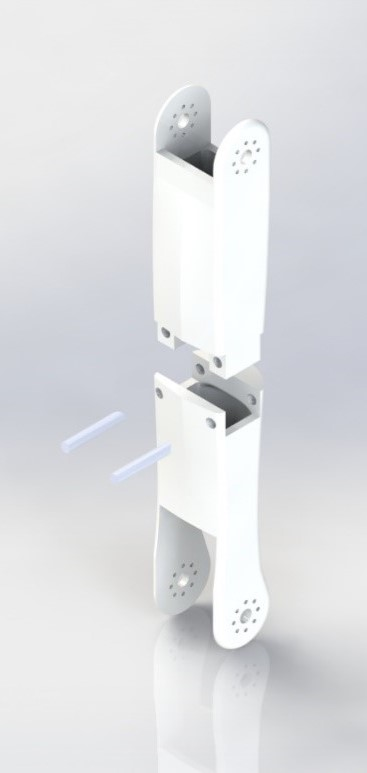
\includegraphics[width=\linewidth]{chapter4/images/shin.jpg}
      \caption{โครงสร้างส่วนหน้าแข้ง}
    \end{subfigure}
    \begin{subfigure}[b]{0.35\linewidth}
      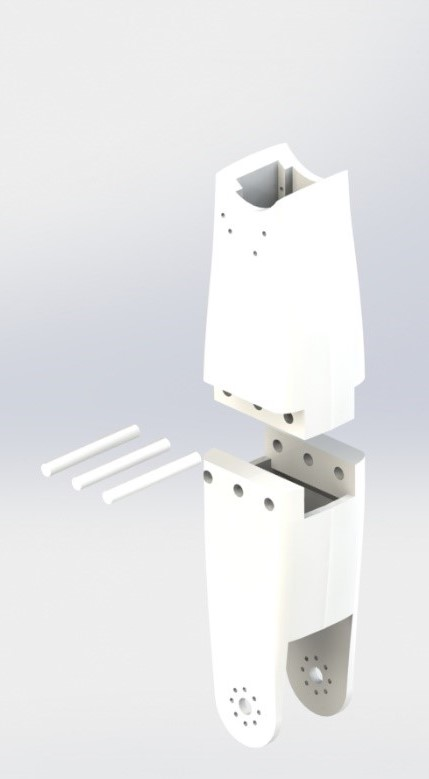
\includegraphics[width=\linewidth]{chapter4/images/thigh.jpg}
      \caption{โครงสร้างส่วนต้นขา}
    \end{subfigure}
    \caption{รูปการออกแบบส่วนขาของหุ่นยนต์อุทัย}
    \label{fig:leg}
  \end{figure}

เมื่อทำการพิมพ์ชิ้นงานส่วนขาท่อนบนและท่อนล่าง ออกมาจะได้น้ำหนักของชิ้นงานตามตาราง \ref{tab:UTHAI_leg}
\begin{table}[ht]
	\centering
	\begin{tabular}{| l | l |}
		\hline
		ชิ้นส่วน & น้ำหนัก(กรัม) \\
        \hline
        ต้นขา & 263 \\
        หน้าแข้ง & 204 \\
	    \hline
	\end{tabular}
	\caption{ตารางแสดงน้ำหนักของชิ้นส่วนขา}
	\label{tab:UTHAI_leg}
\end{table}

จากการทดสอบความสามารถในการเคลื่อนที่ พบว่าตัวขับเคลื่อนสามารถเคลื่อนที่เข้าตำแหน่งได้ถูกต้องตามมุม 
ที่ป้อนเข้าไปให้ระบบ แต่หากทำให้ชิ้นส่วนของขาเคลื่อนที่ด้วยถี่ไปกลับสูงและด้วยความเร็วที่มาก จะทำให้ตัวขับเคลื่อนเกิดการโอเวอร์โหลด 
ซึ่งมีผลทำตัวขับเคลื่อนหยุดการทำงาน ซึ่งต้องทำการปิดเปิดตัวขับเคลื่อนใหม่

จากการทดสอบความแข็งแรงของชิ้นงาน พบว่าชิ้นงานมีความแข็งแรงเพียงพอที่จะทำให้ตัวขับเคลื่อนมีค่าแรงบิดเป็นค่าแรงบิดสูงสุด(Stall Torque)
แล้วทำให้ชิ้นงานไม่เกิดความเสียหาย

จากการทดสอบระยะเวลาการทำงานของตัวขับเคลื่อน ด้วยการเขียนโปรแกรมให้ตัวขับเคลื่อน เคลื่อนที่ไปกลับ สลับตำแหน่งไปเรื่อยๆอย่างต่อเนื่อง เป็นเวลา 20 นาที
พบว่า ตัวขับเคลื่อนทำงานได้เป็นปกติ

\subsubsection*{ปัญหาที่พบในการออกแบบครั้งที่ 1}
เนื่องจากว่าเป้าหมายของการสร้างหุ่นยนต์ตัวนี้ให้มีน้ำหนักที่เบา (น้อยกว่า 5 กิโลกรัม) จึงพบปัญหาว่า
น้ำหนักของส่วนขาที่ได้ออกแบบมานั้นมีน้ำหนักมากเกินกว่าของหุ่นยนต์กนก(ชื่อหุ่นยนต์ตัวเดิมก่อนจะเป็นอุทัย)
ซึ่งเป็นผลทำให้เกิดปํญหาเรื่องภาระโหลดของ motor ที่ต้องกระทำที่มีมากขึ้นจากเดิมและจะทำให้น้ำหนักของตัวหุ่นยนต์มากขึ้น 
เมื่อเปรียบเทียบผลลัพธ์น้ำหนักส่วนขาของหุ่นยนต์กนกกับหุ่นยนต์อุทัยแล้วได้ผลดังตาราง \ref{tab:UTHAI_KANOK_Comp}

\begin{table}[ht]
	\centering
	\begin{tabular}{| l | l | l |}
		\hline
        ชิ้นส่วน & หุ่นยนต์กนก(เดิม)(กรัม) & หุ่นยนต์ UTHAI \\
        \hline
        ขาท่อนบน & 171 & 263 \\
        ขาท่อนล่าง & 172 & 204 \\
	    \hline
	\end{tabular}
	\caption{ตารางเปรียบเทียบน้ำหนักของชิ้นส่วนขาของหุ่นยนต์}
	\label{tab:UTHAI_KANOK_Comp}
\end{table}

จากข้อมูลในตารางนั้นจะเห็นได้ว่า หนักที่เพิ่มขึ้นมากจากการออกแบบใหม่แต่ละชิ้นนั้น มากถึง 124 กรัม
ต่อขา 1 ข้าง และ 248 กรัมเมื่อเทียบกับขาทั้งหมดและเปรียบเทียบกับข้อมูลก่อนหน้า



\subsection{การออกแบบเท้า}
\subsubsection{เซนเซอร์ตรวจจับการสัมผัสพื้น}

\subsection{การออกแบบลำตัว}
\subsubsection{การยึดลำตัวเข้ากับสะโพก}
\subsubsection{การติดตั้งบอร์ดควบคุมและแบตเตอรี่}

\subsection{การออกแบบแขน}



